\chapter{Comparing NoSQL and Relational databases} 
% ! Chapter title doesn't fit the page.


% ? This section "shouldn't be too long, but enough to convince them."
% ! I'm targeting 1000 - 1250 words.
% ? This is NOT comparing *MongoDB* to relational databases.
% ? The brief mentions that it should be "generic just in case after seeing 
% ? your MongoDB database they decide to go with another software provider."

Industrial needs for fast and efficient data storage continue to grow exponentially year by year, and some of these needs fail to be met 
by typical relational database solutions. \textcite{corbelliniPersistingBigdataNoSQL2017} state that the types of data that require storage 
have changed since the first relational database systems of the 1970s, and as such, these more mature systems struggle to meet the requirements of
today's businesses with web-oriented systems storing magnitudes of unstructured data. The same can also be said of Internet of Things 
(IoT) systems, with  \textcite{gubbiInternetThingsIoT2013} stating that 'For the realization of a complete IoT vision, an efficient, secure,
scalable and market oriented computing and storage resourcing is essential.'

\para These efficient, secure and scalable resources exist in the form of NoSQL databases. Chapter 1 provided an overview of NoSQL itself, as well 
as the various types of NoSQL databases, with this chapter instead offering direct comparisons between modern NoSQL solutions to more traditional
relational database management systems in terms of their scalability and transactional models. 


\section{Scalability}
Both \textcite{ganiSurveyIndexingTechniques2016} and \textcite{katalBigDataIssues2013} state that the amount of data stored by companies 
is increasing at an extreme rate, forecasting that companies will likely be storing \textit{zettabytes} of data in the near future.
Because of this, \textcite{gubbiInternetThingsIoT2013}'s previously mentioned efficient and scalable storage solutions are needed to meet 
these ever-increasing demands.

\para Databases can be scaled both vertically and horizontally, with relational databases typically favouring vertical scaling and NoSQL 
databases favouring horizontal scaling, though both are possible in either database type. 

\subsection{Vertical scaling}
Scaling vertically means to upgrade the host device(s) of the database, which refers to the physical swapping or installation of 
parts such as CPUs, RAM and storage drives to accelerate data processing \autocite{cattellScalableSQLNoSQL2011}. 
A significant benefit of a vertically scaled database is that data will always be consistent as it is stored on a single device rather than
distributed across many over a network connection where data could be corrupted, lost or intercepted. This allows for total ACID compliance,
which is described further in Section \ref{subsec:ACID}. 

\para Despite this key benefit, vertical scaling has some downsides. Server components cannot be swapped while the system is online, meaning 
that scaling vertically \textbf{requires} partial or total system downtime, therefore decreasing availability. Furthermore, vertical scaling 
introduces a single point of failure to a system, where the powerful server hosting the database could experience any issue such as a power cut 
that would cause a total system outage. Continuous vertical scaling can also become very costly and bear diminishing returns, with the 
significant cost of top-grade server parts potentially outweighing the performance benefit of their installation 
\autocite{mongodbGuideHorizontalVs}. Vertical scaling also has a fixed limit - a server can only be as good as the best available components.


\subsection{Horizontal scaling}\label{sec:HorizontalScaling}

Scaling horizontally means to add more devices (nodes) to a network, making the database a \textbf{distributed database}. Rather 
than having an entire DBMS stored on a single device and single point of failure, horizontal scaling divides the processing and storage 
loads of the database over many nodes, often through a process called \textbf{sharding}, which involves splitting records into independent 
partitions (shards) based on criteria like ID numbers \autocite{corbelliniPersistingBigdataNoSQL2017}, and replicating these shards over multiple 
nodes. Horizontal scaling is seen almost exclusively with NoSQL databases, as the normalized data models and ACID compliance of relational 
databases mean that scaling horizontally is not feasible \autocite{hechtNoSQLEvaluationUse2011}. 

\para Horizontal scaling introduces considerable benefits for availability, as one node can fail, but the database can continue working 
without it, which allows for maintenance or the addition of extra nodes with minimal to no downtime at all \autocite{mongodbGuideHorizontalVs}.
Furthermore, the aforementioned processing load balancing means that each node doesn't require considerable investment in 
top-grade parts, as nodes can balance processing among themselves. Also, horizontal scaling has no fixed limit unlike vertical scaling, as 
a theoretically infinite amount of nodes can be added dependent on existing network infrastructure, though this would add considerable 
complication to the overall system before long. It is for these reasons that thousands of large enterprises,
including industry titans like Google and Amazon, leverage horizontal scaling of their database systems to maximise their processing speeds
and maximise availability \autocite{changBigtableDistributedStorage2008,amazonModernizingAmazonDatabase2021}. 

\para Despite the wide adoption and considerable benefits, horizontal scaling is not without its own drawbacks. 
Initialising a database with many nodes will introduce a larger initial setup cost, though further upgrades by adding additional nodes 
is typically more cost-effective than scaling vertically as depicted in Figure \ref{fig:ScalingCostOverTime}

\begin{figure}[H]
    \centering
    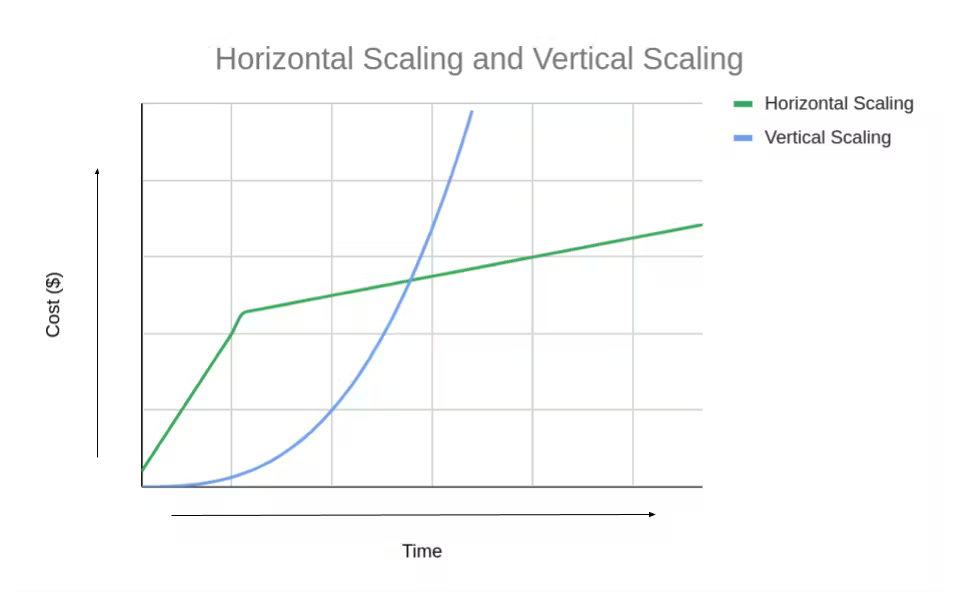
\includegraphics[width=\textwidth]{Comparisons/CostOverTime}
    \caption{An example cost/time graph with each scaling method. \autocite{mongodbGuideHorizontalVs}\label{fig:ScalingCostOverTime}}
\end{figure}


\noindent Additionally, the sharding process relies on \textbf{replication}, meaning that data will be duplicated, reducing storage efficiency
despite the increase in availability. The final considerable drawback is the fact that all nodes are connected via a network, which could 
introduce issues with data transmission, such as the potential for data interception (man-in-the-middle) or corruption (packet loss).

% \para Although horizontal scaling does have these drawbacks, many argue that it remains an overall superior practice to vertical scaling. 
% % ! If you reintroduce this paragrpah, who are the "many"?
% Because horizontal scaling is rarely seen in relational databases, this also means that NoSQL databases will be more useful for large 
% businesses handling considerable amounts of unstructured data.


\section{Transactional models}
Relational and NoSQL databases are governed by dichotomous transactional models that fundamentally change their appropriate use cases.
Relational databases are designed to adhere to the ACID model that prioritises absolute integrity and consistency at the expense of 
both availability and scalability, whereas most NoSQL databases adhere to the opposing BASE model, prioritising availability and scalability
over consistency. However, ACID is not exclusive to relational databases, and recent updates to certain NoSQL databases like MongoDB have 
allowed partial ACID compliance in combination with the scalability benefits of NoSQL.



\subsection{ACID}\label{subsec:ACID}
ACID is an acronym to describe the following key attributes:

% TODO: Talk about ACID:
% ?     Atomicity - A statement is fully executed or not executed at all.
% ?     Consistency - Transactions only occur in predefined ways. (Helps prevent impacts of corruption)
% ?     Isolation - Concurrent transactions don't interfere with each other.
% ?     Durability - Changes are saved, even in the event of system failure. 
% *    https://www.databricks.com/glossary/acid-transactions

\begin{longtable}{ | p{0.2\textwidth} | p{0.7\textwidth} | }
    \hline
    \cellcolor{blue!25}Property & \cellcolor{blue!25}Description\\
    \hline
    Atomicity & All transactions must be fully completed or not completed at all. If a transaction fails,
    the database must be reverted to its prior state with no changes made to the data.  \\
    \hline
    Consistency & Data must meet predefined integrity constraints, and remain consistent for all users even in the event 
    of simultaneous transactions.  \\
    \hline 
    Isolation & Transactions are executed sequentially, and do not interfere with each other even if they are simultaneous. \\
    \hline 
    Durability & Even in the event of system failure, the database must maintain all committed records. This means that 
    even if an error occurs, the results of any and all previous transactions must not be lost. \\
    \hline
    \caption{The key properties of ACID compliance. \autocite{awsACIDVsBASE,neo4jDataConsistencyModels2023}}\label{tab:ACID}
\end{longtable}

\noindent ACID is a very strict model that actively enforces a safe environment for data operations. Though, in maintaining 
such high security, a performance overhead exists with every transaction. This can massively impact the scalability of relational 
databases with complex join operations, which will grow slower the more users they have. 

\para ACID compliance is not exclusive to relational databases, however; in recent years, some NoSQL databases have incorporated ACID 
properties to gain the best of both worlds - high speed and scalability from being non-relational, and high security and integrity from 
ACID compliance. However, NoSQL databases cannot be fully ACID compliant due to their architecture, as horizontal scaling while maintaining 


\subsection{BASE}\label{subsec:BASE}
% TODO: Talk about BASE:
% * A base is the opposite of an acid, hence the name.
% * Seems to be based on the *perception* of availability rather than the literal availability.
% ?     Basically Available - One transaction doesn't have to wait for another to complete first.
% ?     Soft State - The transitional state of records during concurrent updates. Finalised after all transactions complete.
% ?     Eventually Consistent - When all concurrent transactions are done, it will EVENTUALLY be consistent across all user perspectives.
% * https://aws.amazon.com/compare/the-difference-between-acid-and-base-database/

% ! I don't understand transient states and convergence; how can two opposite transactions merge to one eventual state?

BASE-compliant databases operate very differently to their ACID counterparts. Rather than the strict integrity and consistency procedures
expected by ACID, the properties of BASE databases are much more relaxed:

\begin{longtable}{ | p{0.3\textwidth} | p{0.6\textwidth} | }
    \hline
    \cellcolor{blue!25}Property & \cellcolor{blue!25}Description\\
    \hline
    Basically Available & Systems will continue to operate even if failures occur due to redundancy and replication.  \\
    \hline
    Soft State & Replicas do not have to be entirely consistent with each other. This means the system 
    can be in two different states simultaneously, which is known as a transient state.\\
    \hline 
    Eventually Consistent & While updates are not occurring, transient states will converge. \\
    \hline
    \caption{BASE properties. \autocite{corbelliniPersistingBigdataNoSQL2017,cattellScalableSQLNoSQL2011,neo4jDataConsistencyModels2023,awsACIDVsBASE}}\label{tab:BASE}
\end{longtable}

\noindent By forfeiting the strict regulations and associated performance overheads of ACID compliance, BASE-compliant databases can 
theoretically operate at much higher speeds by sacrificing their immediate consistency in favour of eventual consistency and workload
division across many nodes, as was previously noted in Sections \ref{sec:CAPTheorem} and \ref{sec:HorizontalScaling}.

% TODO:
% ?     Overall unhappy with the BASE section. Minimal detail due to lack of understanding which compromises the integrity of the work. 

% ! A very text-heavy section (and CHAPTER, at that.). Add images maybe?
% ! Vertical scaling got two paragraphs but horizontal got a whole page. Consider reducing one or increasing the other.

\section{Overall summary}
In conclusion of all factors discussed across Chapters 1 and 2, the best option for IoThings will be to leverage the heightened capabilities
of a NoSQL database, specifically a \textbf{document store}, to store and query their sensor activation data.

\subsection{Why not a relational database?}
It is unlikely that IoThings will see much benefit from a relational database solution as they require \textbf{high scalability}, which is 
best offered by distributed NoSQL systems. As a home automation company, IoThings will likely be storing sensor readings at regular intervals,
better known as \textbf{time-series data}. If this interval were 30 seconds, and they had 10,000 users, they would be storing 600,000 values 
a minute or 864,000,000 a day. It is not unheard of for this to be done in relational systems, though the previously mentioned lack 
of horizontal scalability of these systems mean that user demand will quickly outpace any vertical scaling that could be performed,
possibly through the sheer storage requirement alone.

\subsection{Why use a document store?}
Based on the specific needs of the company, the best type of NoSQL database to use will be a \textbf{document store}.
Within the document store, JSON/BSON objects each containing the various sensor outputs can be stored and queried with great ease and 
high speed. The programmatic storage of these objects using common types for languages like JavaScript and Python allows for direct 
integration with the IoT device's code, where sensor readings could be directly sent to the DB as part of the device's standard operations,
as document stores excel in storing data of varying types, with time-series data from a thermostat containing the current date and time 
(ISODate type in JavaScript) and temperature (Integer or Double if decimals included) for example. 
One of the software options for this approach, MongoDB, already includes guides for this process in their documentation
\autocite{mongodbModelIoTData}.

% ! Possible colossal error:
% ?     Page 4 of the brief says to compare the relational approach with SPECIFICALLY A DOCUMENT STORE.
% ?     Though later on it then says comparison of relational and NoSQL databases, plural.
% TODO: You will NEED clarification on this, though it doesn't have to come any time soon (report due May 5).
% * I think an optimal approach, while certainly painful to do, would be to keep this file but also make a new one 
% * specifically comparing relational & document, showing how each would store data. That might have been the main intention here.
% * Elements of this could still be kept in that scenario.

% ? Additional note regarding Chapter 1:
% ?     Week 5's lecture says column stores and WIDE column stores are NOT THE SAME.
% ?     Which am I meant to write about in this assignment then?
